\chapter{Samochody autonomiczne}
\label{SDCsChapter}
\vspace{-1cm}
Samochód autonomiczny to \textit{,,pojazd, który potrafi interpretować swoje otoczenie oraz bezpiecznie poruszać się po nim bez potrzeby ingerencji człowieka. Taki pojazd jest zdolny do wykonywania wszelkich manewrów, jakie mógłby wykonać doświadczony kierowca''} \cite{galios:thesis}.
Zgodnie ze skalą zdefiniowaną przez organizację \textit{Society of Automotive Engineers} \cite{synopsys:whatIsAutonomousCar}, w pełni autonomiczne samochody mają być całkowicie pozbawione kierownicy, pedałów oraz innych przyrządów tradycyjnie używanych do sterowania ręcznego. W chwili obecnej nie istnieje ani jeden model takiego samochodu, dopuszczonego do produkcji seryjnej. Co więcej, niewiele wskazuje na to, żeby ten stan rzeczy miał się zmienić w przeciągu kilku kolejnych lat \cite{adams:yearsAwaySDCs, houwelling:wontGetSdcSoon}. Zanim to się wydarzy, inżynierowie oraz badacze zajmujący się tym zagadnieniem będą zmuszeni do rozwiązania jeszcze wielu trudnych problemów technicznych. Oprócz tego dochodzi również kwestia dostosowania przepisów prawnych \cite{businessInsider:autonomiczneAutaPrawo}.

Aby zrozumieć działanie samochodów autonomicznych, należy zapoznać się z czterema kluczowymi elementami zagadnienia:
\begin{enumerate*}
\item \textbf{Percepcja} - pozwala widzieć świat wokół samochodu, jak również rozpoznawać i klasyfikować obiekty pojawiające się w polu widzenia. Aby podejmować dobre decyzje, obiekty powinny być rozpoznawane tak szybko jak to tylko możliwe. Samochód powinien również znać odległości, jakie dzielą go od tych obiektów. Dzięki percepcji samochód wie, czy w danej chwili może przyspieszyć, czy raczej powinien zwalniać. Do obserwacji otoczenia wykorzystuje się 4 typy czujników: czujnik ultradźwiękowy, radar, LiDAR oraz kamerę. Nie zawsze są wykorzystywane wszystkie typy czujników, choć popularnym podejściem jest ich połączone użycie.
\item \textbf{Lokalizacja} - niezbędna do określenia pozycji oraz orientacji samochodu względem innych obiektów obecnych w otaczającej go przestrzeni. Pomaga także w klasyfikacji oraz wizualnej segmentacji obiektów widzianych przez kamerę. Więcej na temat lokalizacji można przeczytać w artykule \cite{nvidia:localisation}.
\item \textbf{Predykcja} - jej zadaniem jest przewidywanie zachowań innych uczestników ruchu drogowego. Model predykcji w głównej mierze opiera się na obliczaniu trajektorii, po jakich poruszają się obiekty w polu widzenia samochodu \cite{singh:prediction}. Trajektorie te pomagają w podejmowaniu odpowiednich decyzji w celu uniknięcia kolizji na drodze.
\item \textbf{Podejmowanie decyzji} - model podejmowania decyzji musi dawać błyskawiczne i precyzyjne wyniki, działając przy tym w środowisku odznaczającym się wysokim poziomem niepewności. Pod uwagę należy brać wiele czynników, takich jak nieracjonalne zachowanie uczestników ruchu lub też zakłócenia pomiarów na skutek usterki jednego z czujników w samochodzie. Celem modelu jest wybór takiego zestawu zachowań, który będzie najbardziej odpowiedni dla danej sytuacji.
\end{enumerate*}

\section{Typy czujników}
Aby widzieć swoje otoczenie, samochody autonomiczne potrzebują urządzeń dostarczających im odpowiednich danych wejściowych. Urządzenia te można ogólnie nazwać czujnikami. Standardowo istnieją cztery typy czujników, jakie można zastosować w samochodzie autonomicznym \cite{petit:sensorFusion}: \textbf{czujnik ultradźwięków}, \textbf{radar}, \textbf{LiDAR} oraz \textbf{kamera}.
Za wyjątkiem kamery, wszystkie pozostałe czujniki wykorzystują tzw. ,,regułę czasu przelotu'' (z ang. \textit{time-of-flight principle}).
Reguła polega na pomiarze odległości od przeszkód oraz prędkości przemieszczania się obiektów na podstawie czasu od emisji sygnału do jego powrotu. Rodzaj sygnału zależy od zastosowanego czujnika - może to być fala ultradźwiękowa, fala radiowa lub wiązka światła. Przykładem zastosowania reguły czasu przelotu jest echolokacja, wykorzystywana m.in. przez nietoperze.

\subsection{Czujnik ultradźwięków}
Korzysta z fali ultradźwiękowej o zadanej częstotliwości. Z powodu specyfiki rozchodzenia się fali ultradźwiękowej w powietrzu, jego zasięg wynosi do kilku metrów, dlatego jest głównie wykorzystywany w systemach \textbf{wspomagania parkowania} oraz \textbf{kontroli martwego pola}.

\subsection{Radar}
Używa fal radiowych, dzięki czemu zasięg jest znacznie większy. Radary są bardzo popularne do pomiarów odległości, natomiast nie nadają się do rozpoznawania obiektów. Jest to spowodowane niską rozdzielczością sygnału. Obecnie w samochodach autonomicznych wykorzystuje się dwa typy radarów:
\begin{enumerate*}
\vspace{-0.5cm}
\item Krótkozasięgowe - do pomiarów na krótkim dystansie, tj. do 30 metrów. Fala radiowa ma częstotliwość ok. 24 GHz. Zalety rozwiązania to niska podatność na zakłócenia oraz niskie koszty produkcji.
\item Długozasięgowe - do wykonywania pomiarów na dystansie do 250 metrów. Częstotliwość fali radiowej waha się pomiędzy 76 a 77 GHz. 
\end{enumerate*}

\subsection{LiDAR}
Nazwa to akronim od angielskiego wyrażenia \textit{\textbf{Li}ght \textbf{D}etection \textbf{a}nd \textbf{R}anging}. Pomiarów można dokonywać na krótkich i długich dystansach. Główną zaletą tej technologii jest generowanie danych 3D o wysokiej rozdzielczości, albowiem LiDAR emituje setki tysięcy impulsów laserowych na sekundę. Największe wady LiDAR-u to wysoka cena oraz wysoka podatność na warunki pogodowe - działanie czujników ulega znaczącemu pogorszeniu pod wpływem deszczu, śniegu lub mgły.

\subsection{Kamera}
Kamera dla maszyny jest tym, czym oko dla człowieka - pozwala widzieć otaczający świat. We współczesnych samochodach autonomicznych jest to niezbędny element wyposażenia. Kamera jako jedyna dostarcza informacji o kolorach, jest również nieocenioną pomocą przy identyfikacji oraz klasyfikacji obiektów należących do otoczenia. Odczytywanie znaków drogowych lub ostrzeganie przed niezamierzonym zjazdem ze swojego pasa byłoby niemożliwe bez wykorzystania kamery.

Niemniej jednak, nie jest to rozwiązanie pozbawione wad - na jej działanie mają wpływ warunki pogodowe, jak również pojedyncza kamera nie dostarcza informacji o głębi obrazu. Aby uzyskać obraz 3D, wymagane jest użycie co najmniej dwóch kamer.

\section{Kamera kontra LiDAR}
Od kilku lat w środowisku osób zajmujących się rozwojem technologii samochodów autonomicznych trwa zagorzała dyskusja. Co jest lepsze - kamera czy LiDAR? Prezentowane są różne stanowiska, a przytaczane argumenty za i przeciw dla każdego z rozwiązań utrwalają w przekonaniu, iż temat nie jest trywialny i wart jest dokładniejszego przyjrzenia się. Dlatego też w niniejszym podrozdziale postanowiłem pokrótce omówić te zagadnienie \cite{autopilotReview:lidarVsCamera}, przedstawiając zalety i wady każdego z rozwiązań.

\subsection{LiDAR - zalety}
Zwolennicy LiDAR-u wskazują na jego wysoką dokładność oraz precyzję. System LiDAR opracowany przez firmę Waymo jest tak zaawansowany, że potrafi rozpoznawać oraz przewidywać kierunek, w jakim mogą podążać piesi.

Inną zaletą LiDAR-u jest generowanie obrazu 3D bezpośrednio z danych otrzymanych z czujnika. LiDAR jest pod tym względem bardziej dokładny w porównaniu do kamery, ponieważ jego działanie nie będzie zakłócane zmiennym oświetleniem otoczenia.

Kolejnym argumentem jest znacznie mniejsze zapotrzebowanie na moc obliczeniową niż ma to miejsce w przypadku użycia kamery. Dzieje się tak, ponieważ bezpośrednio z danych wejściowych dostarczanych przez LiDAR da się wyciągnąć wiele informacji o przestrzeni wokół samochodu. Te same informacje w przypadku użycia kamery muszą zostać wygenerowane przez komputer.

\subsection{LiDAR - wady}
Wskazując wady LiDAR-u, należy wspomnieć o kilku kwestiach. Pierwszą z nich jest cena - systemy LiDAR były kiedyś bardzo drogie. Oryginalnie używany przez firmę Google zestaw czujników LiDAR dla pojedynczego samochodu kosztował powyżej 75 000 dolarów. Dziś ceny czujników LiDAR są znacznie niższe, niemniej jednak wciąż są wysokie.

Kolejna wada to zakłócanie sygnału, do jakiego dochodzi gdy w pobliżu siebie znajdą się co najmniej dwa samochody wyposażone w system LiDAR. Im więcej samochodów jednocześnie generujących impulsy świetlne, tym większe ryzyko ,,oślepienia'' innych pojazdów. Producenci będą musieli jakoś temu zaradzić.

Nieznane są również długofalowe skutki pernamentnej ekspozycji na wiązki laserowe generowane przez system LiDAR. Obawy dotyczą zwłaszcza narządu wzroku człowieka \cite{armenta:lidarSafety, thomasAko:lidarSafety, hecht:lidarSafety}.

Kolejnym ograniczeniem systemu LiDAR jest pogorszone działanie przy niekorzystnych warunkach pogodowych, takich jak deszcz, śnieg czy mgła. Krople deszczu mogą być przez system interpretowane jako ściana na środku drogi. Niektóre firmy (np. Ford) radzą sobie z tym problemem poprzez opracowanie własnych algorytmów wspomagających interpretację sygnału pobieranego z czujników LiDAR. Niemniej jednak, są to rozwiązania niedojrzałe i wymagające dalszego dopracowania.

Ostatnim palącym problemem jest niemożliwość dostarczenia informacji, które można bez problemu uzyskać z obrazu kamery. Do tych informacji należy m.in. oznakowanie drogi (pionowe i poziome) oraz kolory świateł na skrzyżowaniach.

\subsection{Kamera - zalety}
Po pierwsze, kamery są znacznie tańsze od systemów LiDAR, co przekłada się na większą dostępność dla konsumentów. Są również łatwiejsze do wdrożenia, ponieważ kamery jako urządzenia są bardzo szeroko dostępne na rynku.

Po drugie, samochód wyposażony w kamery znacznie lepiej radzi sobie w trudnych warunkach pogodowych (deszcz, śnieg, mgła) niż ma to miejsce w przypadku samochodu z systemem LiDAR.

Po trzecie, kamery potrafią widzieć świat tak samo jak widzą go ludzie, zatem są w stanie rozpoznawać kolory, oznakowania dróg oraz wiele innych elementów otoczenia.

Ostatnia zaleta jest taka, że kamery da się dużo łatwiej zabudować w nadwozie w taki sposób, aby nie psuć ogólnej estetyki samochodu. Dzięki temu znacznie więcej potencjalnych klientów może być zainteresowana zakupem takiego pojazdu.

\subsection{Kamera - wady}
Kamery są narażone na te same problemy, co ludzkie oko - jazda po słabo oświetlonym terenie lub ostre, oślepiające światło świecące prosto w kamerę mogą powodować zakłócenia w rozpoznawaniu otoczenia. W takich przypadkach samochód nie zawsze jest w stanie podejmować właściwe decyzje na drodze.

Kolejną wadą jest fakt, że surowe dane z kamery są mało użyteczne, ponieważ każda zarejestrowana klatka obrazu jest tylko zlepkiem pikseli o określonym zagęszczeniu. Aby dane pochodzące z kamery mogły być wykorzystane, muszą zostać przetworzone przez odpowiednie oprogramowanie. Do stworzenia takiego oprogramowania jest wymagana zaawansowana wiedza z zakresu sieci neuronowych oraz głębokiego uczenia maszynowego, a także wielka ilość danych potrzebnych do treningu sieci.

Kolejny problem to moc obliczeniowa, niezbędna do przetwarzania w czasie rzeczywistym ogromnej ilości danych generowanych z kamer samochodu podczas jazdy. Przetwarzanie danych nie może przekraczać zakładanych limitów czasowych, ponieważ w przeciwnym razie mogłoby to wpływać na bezpieczeństwo jazdy. Ilość generowanych danych także nie może być znacząco zredukowana, ponieważ trzeba zachować niezbędne minimum w zakresie liczby klatek na sekundę oraz rozdzielczości obrazów wejściowych. Aby stawić czoła tym wyzwaniom, projektowane są specjalne platformy sprzętowe do wykorzystania w samochodach autonomicznych. Przykładem takiej platformy jest \textit{Full Self-Driving Computer}, zaprezentowany przez firmę Tesla w 2019 roku \cite{autopilotReview:fsdComputer}.

\subsection{Podsumowanie}
Po zapoznaniu z argumentami obydwu stron wydaje się, że bardziej przyszłościowym rozwiązaniem dla samochodów autonomicznych może być rezygnacja z dalszego użycia technologii LiDAR i skupienie się na rozwoju oprogramowania przetwarzającego obraz z kamer zamontowanych w pojeździe. Uważa tak również wiele wybitnych osób zajmujących się tym tematem, a jednym z ich najgłośniejszych przedstawicieli jest Elon Musk. Wielokrotnie krytykował stosowanie systemu LiDAR w samochodach autonomicznych, uważając to za ślepy zaułek \cite{burns:elonMuskLidar}. Z drugiej strony, choć docelowo Elon Musk może mieć rację, to przy obecnym stanie rozwoju oprogramowania LiDAR wciąż wydaje się być atrakcyjną opcją, co zostało bardzo dobrze opisane w artykule \cite{forbes:muskWarOnLidar}. Istnieje bowiem wiele sytuacji, w których LiDAR wciąż daje lepsze efekty niż systemy oparte wyłącznie na obrazie z kamer.

\section{Rozwiązania wiodące na rynku}
W chwili obecnej wiele korporacji o międzynarodowych zasięgach inwestuje ogromne środki w rozwój technologii samochodów autonomicznych. Niniejsze zestawienie jest subiektywną listą najciekawszych rozwiązań obecnych na rynku. Zaprezentowane rozwiązania zostały przez autora wybrane ze względu na fakt, że charakteryzują się one najwyższym stopniem zaawansowania i dają najlepsze perspektywy na rozwój technologii w przyszłości.

\subsection{Waymo Driver}
Waymo zostało założone w 2009 r. jako projekt firmy Google, później stało się przedsiębiorstwem technologicznym wchodzącym w skład holdingu Alphabet Inc. Waymo zajmuje się rozwijaniem technologii samochodów autonomicznych. Ich obecny system autonomicznej jazdy samochodem nosi nazwę \textbf{Waymo Driver} i jest stawiany w gronie najbardziej dojrzałych i przetestowanych rozwiązań, ponieważ samochody Waymo mają na swoim koncie ponad 20 milionów mil przejechanych w prawdziwym świecie i ponad 20 miliardów mil przejechanych w symulacji komputerowej. Trening oraz testy odbywały się w możliwie najszerszym spektrum warunków pogodowych oraz rozpatrywanych scenariuszy drogowych.

Samochód do jazdy po danym regionie potrzebuje precyzyjnych oraz szczegółowych map 3D, posiadających szereg informacji, takich jak profile dróg oraz wszystkie elementy pionowego i poziomego oznakowania.

Obecna, piąta generacja systemu \textbf{Waymo Driver} wykorzystuje trzy typy czujników: kamerę, radar oraz LiDAR \cite{waymoDriver:5thGenSensors}. Układ czujników został zaprezentowany na rysunku \ref{WaymoDriverSensors}. \\

\begin{figure}[h]
\begin{center}
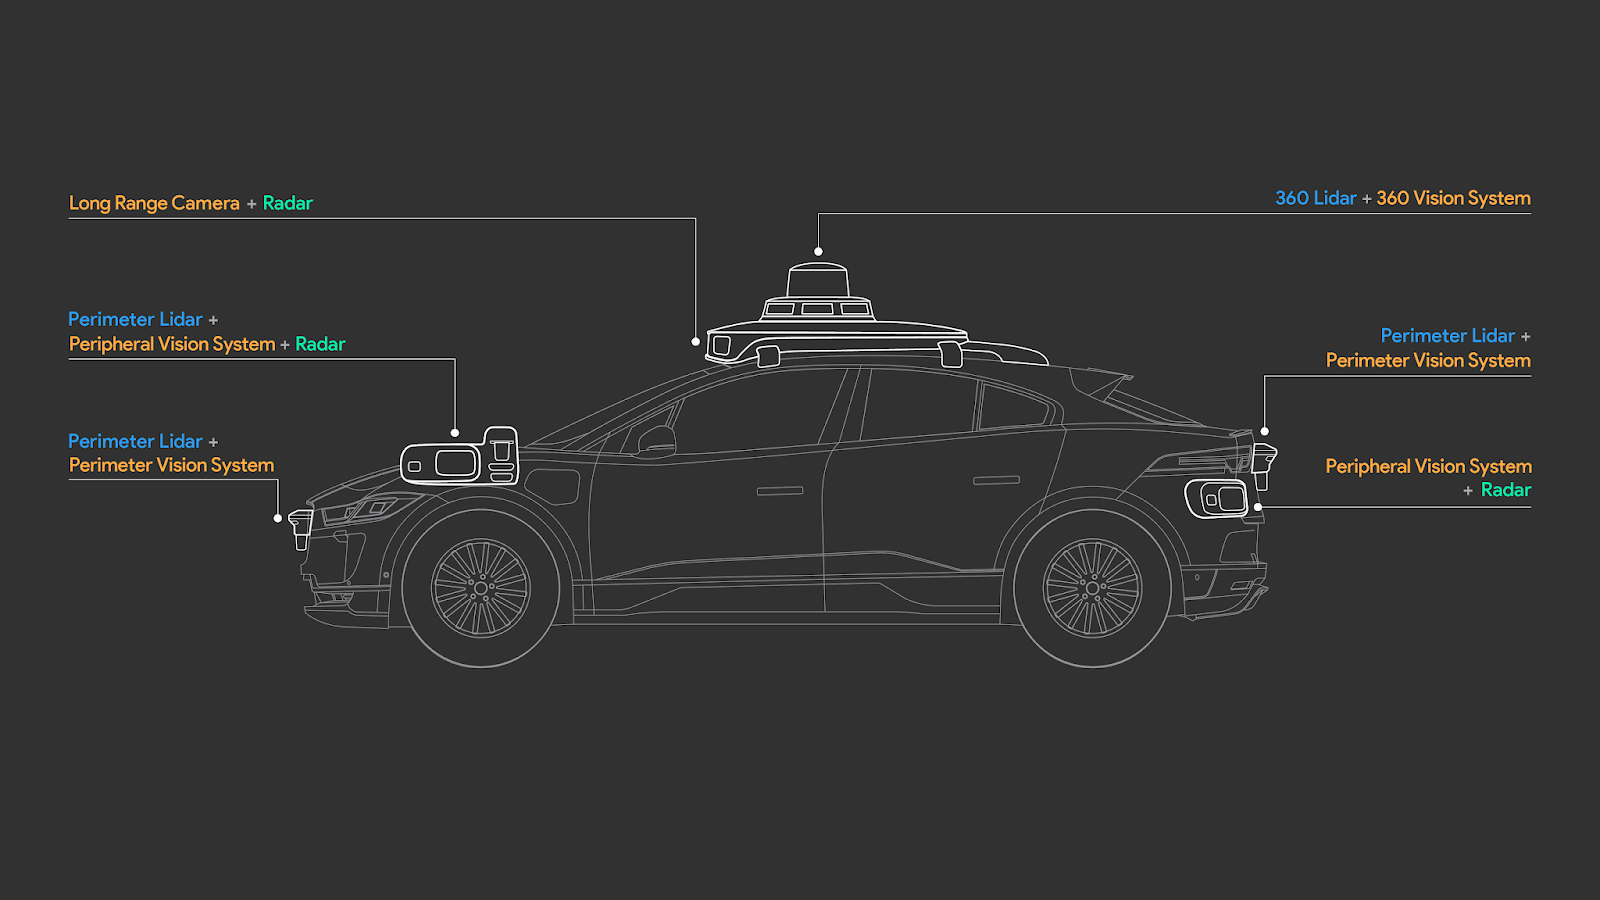
\includegraphics[width=15cm]{resources/figures/waymo_driver_sensors.png}
\caption{Układ czujników systemu Waymo Driver}
\source{https://blog.waymo.com/2020/03/introducing-5th-generation-waymo-driver.html}
\label{WaymoDriverSensors}
\end{center}
\end{figure}

Czujniki LiDAR mają wysoką rozdzielczość i zasięg do 300 metrów. Kamery dają bardzo ostry obraz o dobrej jakości. System widzenia obwodowego działa we współpracy z systemem LiDAR-ów obwodowych (z ang. \textit{perimeter lidars}), dzięki czemu samochód lepiej widzi co się dzieje w jego najbliższym otoczeniu - to pomaga w wielu sytuacjach, na przykład podczas manewrów parkowania. Radary wspomagają pracę czujników LiDAR w trudnych warunkach pogodowych, odznaczają się także wysoką rozdzielczością i zasięgiem rzędu kilkuset metrów.

\subsection{NVIDIA DRIVE}
Firma NVIDIA od dawna inwestuje w rozwój technologii samochodów autonomicznych. Więcej informacji na ten temat można znaleźć w pracy \cite{galios:thesis}. Znajdujący się tam opis systemu NVIDIA DRIVE jest wciąż aktualny, dlatego autor pracy postanowił nie powielać go tutaj.

\subsection{Tesla Autopilot}
Firma Tesla zasłynęła produkcją swoich samochodów elektrycznych. Opracowała również zaawansowany system wspomagania jazdy, noszący nazwę \textbf{Tesla Autopilot} \cite{tesla:autopilotOverview}. System został stworzony w celu zwiększenia bezpieczeństwa oraz komfortu podróżowania kierowcy, pasażerów oraz innych uczestników ruchu drogowego. Każdy nowy samochód Tesli wyposażony jest w osiem kamer, a samochody sprzedawane poza Ameryką Północną są również wyposażone w zestaw czujników radarowych. Autopilot nie zapewnia pełnej autonomii samochodu, dlatego kierowca musi zachować stałą czujność podczas jazdy i być gotów przejąć kontrolę nad sterowaniem, gdy zajdzie taka potrzeba.

W skład Autopilota wchodzą następujące funkcje:
\begin{enumerate*}
\item \textbf{Traffic-Aware Cruise Control} - dopasowuje prędkość samochodu do otaczającego ruchu ulicznego;
\item \textbf{Autosteer} - wspomaga kierowanie na drodze posiadającej wyraźnie oznaczone pasy ruchu oraz wykorzystuje aktywny tempomat, który uwzględnia ruch drogowy wokół samochodu.
\end{enumerate*}

Tesla ma także w swojej ofercie pakiet rozszerzeń \textbf{Full Self-Driving Capability}, który wzbogaca Autopilota o takie funkcje jak:
\vspace{-0.25cm}
\begin{enumerate*}
\item \textbf{Navigate on Autopilot} - umożliwia półautonomiczną jazdę po autostradzie.
\item \textbf{Auto Lane Change} - pomaga w zmianie pasa ruchu na autostradzie, gdy jest włączona funkcja \textbf{Autosteer}.
\item \textbf{Autopark} - pomaga zaparkować samochód (równolegle lub prostopadle).
\item \textbf{Summon} - wprowadza oraz wyprowadza samochód z ciasnej przestrzeni za pomocą aplikacji mobilnej.
\item \textbf{Smart Summon} - samochód nawiguje po skomplikowanych obiektach typu place parkingowe, aby odnaleźć kierowcę i podjechać do niego.
\item \textbf{Stop Sign and Traffic Light Control} - pierwsza funkcja przeznaczona do użytku w ruchu miejskim. Pojazdy Tesli wyposażone w tę funkcję potrafią reagować na znaki stop oraz sygnalizację świetlną. Przy dojeżdżaniu do skrzyżowania ze światłami samochód zwalnia (nawet mając zielone), a kierowca musi nacisnąć pedał przyspieszenia. Wtedy samochód kontynuuje jazdę w trybie automatycznym.
\end{enumerate*}

Samochody Tesli są również wyposażone w zestaw aktywnych funkcji bezpieczeństwa:
\vspace{-0.25cm}
\begin{enumerate*}
\item \textbf{Automatic Emergency Braking} - wykrywa przeszkody, w które samochód mógłby uderzyć i odpowiednio do sytuacji uruchamia hamulce;
\item \textbf{Forward Collision Warning} - ostrzega przed nadciągającą kolizją z wolniej poruszającymi się samochodami;
\item \textbf{Side Collision Warning} - ostrzega przed potencjalną kolizją z obiektami rozmieszczonymi wokół samochodu;
\item \textbf{Obstacle Aware Acceleration} - automatycznie zmniejsza przyspieszenie samochodu po wykryciu przeszkody podczas jazdy z małą prędkością;
\item \textbf{Blind Spot Monitoring} - ostrzega przed obiektami w martwym polu, gdy samochód wykonuje manewr zmiany pasa;
\item \textbf{Lane Departure Avoidance} - stosuje manewry korygujące w celu utrzymania się na swoim pasie ruchu;
\item \textbf{Emergency Lane Departure Avoidance} - przywraca pojazd z powrotem na swój pas ruchu, gdy wykrywa że samochód zjeżdża ze swojego pasa i może dojść do kolizji na drodze.
\end{enumerate*}

\subsubsection{Tesla Vision}
Tesla jest obecnie liderem na rynku pod względem rozwoju technologii wykorzystania kamer w samochodach autonomicznych. Ich system o nazwie 
\textbf{Tesla Vision} to nowa wersja systemu \textbf{Tesla Autopilot}, w której całą percepcję oparto tylko na jednym typie czujnika: kamerze. Począwszy od maja 2021, system ten jest montowany w samochodach Tesli sprzedawanych w Ameryce Północnej \cite{tesla:transToVision}.

Pomysł całkowitej rezygnacji z radarów oraz LiDAR-ów wzbudził wiele kontrowersji w środowisku osób zainteresowanych rozwojem technologii samochodów autonomicznych. W dość obszernym artykule \cite{torchinsky:teslaRemoveRadar} z maja 2021 roku, autor wysuwa szereg trafnych argumentów przeciwko decyzji Tesli o rezygnacji z montowania radarów w niektórych ich modelach. Radary doskonale uzupełniają dane z kamer, zwłaszcza w sytuacji kiepskiej widoczności na drodze. Z radarami łatwiej jest generować trójwymiarową reprezentację otoczenia samochodu, ponieważ uzyskujemy ją bezpośrednio z odczytów radaru (w przeciwieństwie do obrazu z kamery, gdzie informacja o głębi musi zostać obliczona przez oprogramowanie pojazdu). Sygnał z radarów jest w stanie prześlizgnąć się i wrócić pod samochodami jadącymi bezpośrednio przed samochodem autonomicznym, dzięki czemu samochód może zareagować z większym wyprzedzeniem i uniknąć kolizji, do której doszłoby w innym wypadku.

Autora nie przekonują argumenty typu ,,\textit{człowiek też nie ma radarów i jakoś sobie radzi z prowadzeniem samochodu}'', ponieważ ignorują one fundamentalny problem, jaki przeszkadza w osiągnięciu pełnej autonomii pojazdu: nasze oprogramowanie wciąż jest bardzo dalekie od tego, co potrafi ludzki mózg. Dotyczy to zarówno umiejętności sprawnego interpretowania obrazów, jak również logicznego rozumowania oraz zdolności adaptacji do nowego środowiska i radzenia sobie w niestandardowych scenariuszach drogowych. Na każdym z tych pól oprogramowanie wykazuje poważne braki i niedociągnięcia w stosunku do możliwości człowieka. Skoro Tesla nie wprowadziła żadnej rewolucji w tym zakresie, to pozbycie się radarów dających cenne źródło informacji należy uznać za regresję w możliwościach systemu. Zwłaszcza, że nie wprowadzono żadnej redundancji w postaci dodatkowych kamer, dlatego też przy awarii chociaż jednej z nich lub nawet zasłonięciu soczewki (np. z powodu zalegającego śniegu lub ptasich odchodów), percepcja samochodu ulega znaczącemu pogorszeniu.

Pomimo powyższych zastrzeżeń wygląda na to, że Tesla nieustannie doskonali swój produkt i wraz z kolejnymi aktualizacjami oprogramowania ich samochody radzą sobie coraz lepiej - również w trudnych warunkach pogodowych, co zostało opisane w artykule \cite{klender:teslaOnHeavyRain}. Autor przedstawił odczucia jednego z użytkowników samochodu Tesli, który zauważał postępującą poprawę zachowania samochodu podczas jazdy w intensywnym deszczu. Poprawa ta następowała (w mniejszym lub większym stopniu) po każdej aktualizacji oprogramowania i objawiała się mniejszym i mniej gwałtownym wytracaniem prędkości pojazdu.

Podczas konferencji CVPR z 2021 roku, Andrej Karpathy (szef działu AI w Tesli) wyjaśnił dlaczego Tesla zrezygnowała z wykorzystania czujników LiDAR w swoich samochodach \cite{dickson:teslaDontNeedLidar}. Karpathy wskazał między innymi na problem przygotowania i utrzymania dokładnych i szczegółowych map 3D terenu, po którym ma się poruszać samochód wyposażony w czujniki LiDAR. ,,\textit{Musisz wstępnie zmapować środowisko za pomocą LiDAR-u, a następnie stworzyć mapę w wysokiej rozdzielczości i wstawić tam wszystkie pasy i sygnalizacje świetlne}'' - powiedział Karpathy. Dodał również: ,,\textit{Zbieranie, budowanie i utrzymywanie map LiDAR-owych w wysokiej rozdzielczości jest nieskalowalne. Bardzo trudno utrzymać tę infrastrukturę w stanie aktualnym}''. Samochody Tesli nie potrzebują mieć ręcznie przygotowanych map 3D, ponieważ same potrafią wygenerować sobie takie mapy. ,,\textit{Wszystko co się dzieje, dzieje się po raz pierwszy w samochodzie, na podstawie nagrań z ośmiu kamer otaczających samochód}'' - stwierdził Andrej Karpathy. Samochód musi samodzielnie rozpoznać otoczenie, wykryć i zinterpretować wszystkie elementy infrastruktury drogowej oraz ocenić, które z nich są dla niego istotne. Wszystko to bez jakiejkolwiek wcześniejszej informacji na temat drogi, po której samochód będzie się przemieszczać.

\subsubsection{Platforma sprzętowa}
Dodatkowym warunkiem, jaki musi spełniać samochód autonomiczny, jest maksymalny dopuszczalny czas obliczeń podczas jazdy samochodem. Wszystko musi odbywać się w czasie rzeczywistym, a zbyt wielkie opóźnienia w przetwarzaniu danych mogłyby doprowadzić do wystąpienia niebezpiecznej sytuacji na drodze. Na szczęście Tesla dysponuje bardzo dobrym sprzętem, opracowanym we współpracy z firmą Samsung \cite{wiggers:teslaDrivingChip, autopilotReview:fsdComputer}. Nosi nazwę \textbf{Full Self-Driving Computer} (FSD) i w momencie swojej premiery w 2019 roku był określany jako ,,\textit{najbardziej zaawansowany komputer przeznaczony do jazdy autonomicznej}''. Wygląd komputera został zaprezentowany na rysunku \ref{TeslaFsdHardware}.

\begin{figure}[h]
\begin{center}
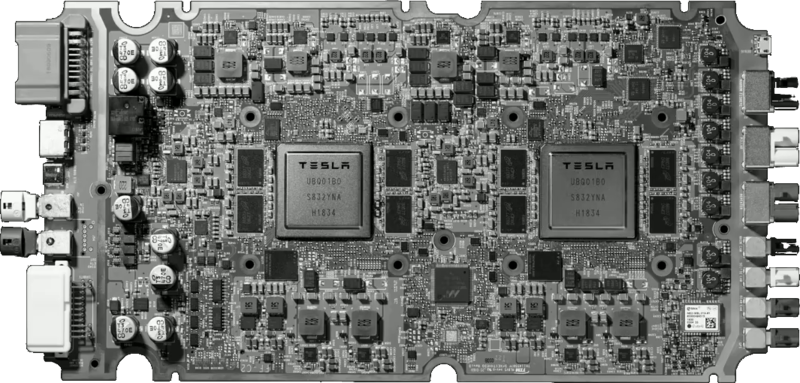
\includegraphics[width=13.5cm]{resources/figures/tesla_fsd.png}
\caption{Komputer Tesla FSD}
\source{https://www.autopilotreview.com/tesla-custom-ai-chips-hardware-3}
\label{TeslaFsdHardware}
\end{center}
\vspace{-1cm}
\end{figure}

Chipset Samsunga osiąga wydajność 144 TOPS i składa się z dwóch redundantnych, niezależnych pakietów - każdy z nich dysponuje własną pamięcią DRAM, układami pamięci flash oraz zasilaniem. ,,\textit{Każdy z pakietów uruchamia i utrzymuje własną instancję systemu operacyjnego}'' - mówi Pete Bannon, projektant układów scalonych pracujący dla Tesli. Dwa pakiety niezależnie od siebie dokonują obliczeń akcji do wykonania, a następnie wymieniają się ze sobą wynikami obliczeń. Żadna akcja nie zostanie zlecona do wykonania kontrolerom samochodu do czasu jej uzgodnienia i zatwierdzenia przez obydwa pakiety. Układ zachowuje swoją zdolność działania także wtedy, gdy jeden z pakietów (lub któraś z jego części) ulegnie awarii. Elon Musk stwierdził, że: ,,\textit{nawet jeśli część układu ulegnie awarii, samochód wciąż może kontynuować jazdę}''.

FSD składa się z 6 miliardów tranzystorów i 250 milionów bramek logicznych. Jego moduły pamięci LPDDR4 RAM zapewniają przepustowość 68 GB/s, a zintegrowane procesory przetwarzania obrazów pracują z prędkością do 1 gigapiksela na sekundę. Dodatkowo w zestawie są dwa akceleratory sieci neuronowych, taktowane z częstotliwością 2 GHz i wyposażone w 32 MB pamięci SRAM. Akceleratory mogą dodawać macierze oraz przetwarzać do 1 TB danych na sekundę, a ich wydajność wynosi 36 TOPS dla każdego z nich (czyli łącznie 72 TOPS). Innym ważnym komponentem jest wbudowany układ zabezpieczający, którego zadaniem jest blokowanie kodu nieposiadającego podpisu kryptograficznego Tesli.

Podczas testów zamkniętych, przeprowadzonych przez firmę Tesla, okazało się że komputer FSD jest w stanie przetwarzać 2300 klatek na sekundę - podczas gdy poprzednia generacja komputera osiągała zaledwie 110 klatek na sekundę.

\subsubsection{Podsumowanie}
Tesla Autopilot to niezwykle ciekawy i wyróżniający się na tle konkurencji projekt. Przedstawiciele Tesli wnieśli ważny głos do dyskusji nad rozwojem technologii samochodów autonomicznych, zwłaszcza w konteście wykorzystania obrazu z kamery jako głównego źródła danych dla modelu percepcji pojazdu. Wkład firmy w rozwój technologii jest bezcenny, nawet jeśli zastosowane podejście okaże się ślepym zaułkiem w drodze do osiągnięcia w pełni autonomicznego systemu sterowania samochodem.